\documentclass[11pt,
			   %10pt, 
               %hyperref={colorlinks},
               aspectratio=169,
               hyperref={colorlinks}
               ]{beamer}
\usetheme{Singapore}
\usecolortheme[snowy, cautious]{owl}

\usepackage[utf8]{inputenc}
\usepackage[T1]{fontenc}
\usepackage[american]{babel}
\usepackage{graphicx}
\usepackage{hyperref}
\hypersetup{
    colorlinks=true,
    urlcolor=[rgb]{1,0,1},
    linkcolor=[rgb]{1,0,1}}

\usepackage[natbib=true,style=authoryear,backend=bibtex,useprefix=true]{biblatex}
\usepackage{listings}
\lstset{numbers=right, 
        numberstyle=\tiny, 
%        breaklines=true,
%        backgroundcolor=\color{light-gray},
        numbersep=5pt,
	xleftmargin=\parindent,
	xrightmargin=.25in} 

%\setbeamercolor*{bibliography entry title}{fg=black}
%\setbeamercolor*{bibliography entry location}{fg=black}
%\setbeamercolor*{bibliography entry note}{fg=black}
\definecolor{OwlGreen}{RGB}{75,0,130} % easier to see
\setbeamertemplate{bibliography item}{}
\setbeamerfont{caption}{size=\footnotesize}
\setbeamertemplate{frametitle continuation}{}
\setcounter{tocdepth}{1}
\renewcommand*{\bibfont}{\scriptsize}
\addbibresource{bibliography.bib}

\renewcommand*{\thefootnote}{\fnsymbol{footnote}}

%\author{\copyright\hspace{1pt}Ashrith Barthur\footnote{\tiny{This material is shared under a \href{https://creativecommons.org/licenses/by/4.0/deed.ast}{CC By 4.0 license} which allows for editing and redistribution, even for commercial purposes. However, any derivative work should attribute the author and H2O.AI.}}}
\author{Ashrith Barthur}
\title{Detecting Money Laundering FP with AI}
\subtitle{Building Machine Learning Recipes to Detect Malicious Behaviours}
\logo{
\includegraphics[height=8pt]{img/h2o_logo.png}}
\institute{\href{https://www.h2o.ai}{H\textsubscript{2}O.ai}}
\date{\today}
\subject{Detecting Money Laundering FP with AI}

\begin{document}
	
	\maketitle
	
	\begin{frame}
	
		\frametitle{Contents}
		
		\tableofcontents{}
		
	\end{frame}

%-------------------------------------------------------------------------------
%	\section{Thanks}
%-------------------------------------------------------------------------------
	\begin{frame}
		\frametitle{Thanks}
		\begin{enumerate}
			\item Audience
			\item Our Customers
			\item AI4 Team
			\item H2O Team
			\item Patrick Hall - Thanks for the beamer template.
		\end{enumerate}
	\end{frame}

%-------------------------------------------------------------------------------
%	\section{Speaker}
%-------------------------------------------------------------------------------
	\begin{frame}
		\frametitle{Speaker}
		\begin{enumerate}
			\item Principal Security Scientist at H2O.AI.
			\item Researcher in the area of anomalies specific to malicious behaviour, graduated with a PhD from Purdue. 
			\item Areas -  Cybersecurity, Electronic Fraud, Money Laundering, and Global Malicious Migratory Patterns.
			\item When I am not working, I am usually biking, or taking pictures. 
			\item @ashrith (github) @cyberbaggage (twitter) @ba(h2o.ai)
		\end{enumerate}
	\end{frame}

%-------------------------------------------------------------------------------
\section{Overview}
%-------------------------------------------------------------------------------
	\begin{frame}
		\frametitle{Question}
		How many of us attending today's webinar analyse data and build models?
	\end{frame}

%-------------------------------------------------------------------------------
%	\section{Overview}
%-------------------------------------------------------------------------------
	\begin{frame}
		\frametitle{Overview}

		This presentation introduces us to three topics. These topics are:
		\begin{enumerate}
			\item An introduction to Detecting False Positive in Money Laundering Alerts using feature recipes. 
			\item A simple, starter guide to building your own feature recipes. 
			\item A 'peek' introduction to detecting malicious behaviours. Malicious Domains in cybersecurity.
		\end{enumerate}
	\end{frame}

%-------------------------------------------------------------------------------
%	\section{H2O.AI Overview}
%-------------------------------------------------------------------------------
	\begin{frame}
		\frametitle{Question} 
		How many of the people attending today have known about H2O.AI?
	\end{frame}


%-------------------------------------------------------------------------------
%	\subection{H2O.AI Overview Team}
%-------------------------------------------------------------------------------
	\begin{frame}
		\frametitle{H2O.AI Overview}
		\begin{figure}[htb]
			\begin{center}
				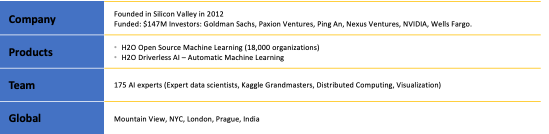
\includegraphics[width=0.95\textwidth]{img/team.png}
				\label{fig:team}
			\end{center}
		\end{figure}
	\end{frame}
%-------------------------------------------------------------------------------
%\subsection{H2O.AI Overview Areas}
%-------------------------------------------------------------------------------
	\begin{frame}
		\frametitle{Industry Footprint}
		\begin{figure}[htb]
			\begin{center}
				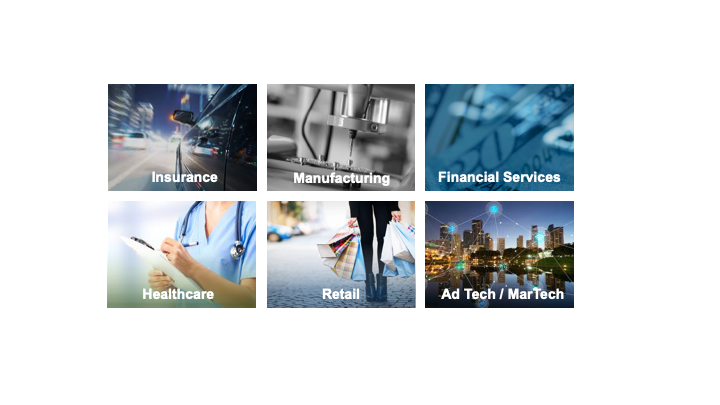
\includegraphics[width=0.95\textwidth]{img/industry.png}
				\label{fig:industry}
			\end{center}
		\end{figure}
	\end{frame}

%-------------------------------------------------------------------------------
%\section{H2O.AI Overview}
%-------------------------------------------------------------------------------
	\begin{frame}
		\frametitle{Question} 
		How many of the people attending today have known, or used Driverless AI?
	\end{frame}

%-------------------------------------------------------------------------------
%\section{DAI}
%-------------------------------------------------------------------------------
	\begin{frame}
		\frametitle{Driverless AI}
		\begin{figure}[htb]
			\begin{center}
				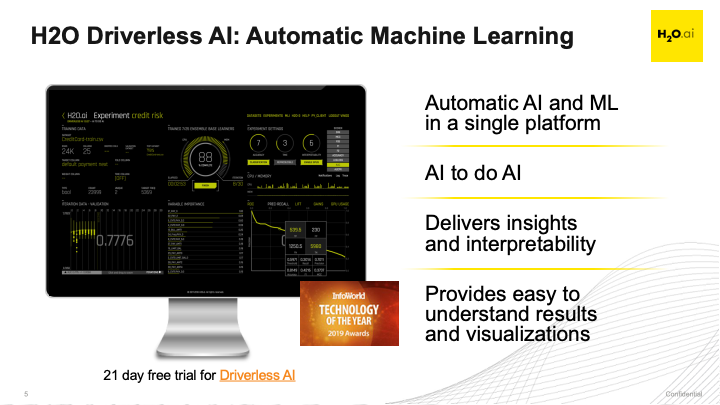
\includegraphics[width=0.75\textwidth]{img/dai.png}
				\label{fig:dai}
			\end{center}
		\end{figure}
	\end{frame}
%-------------------------------------------------------------------------------
\section{Anti Money Laundering}
%-------------------------------------------------------------------------------
%-------------------------------------------------------------------------------
	\subsection{Anti Money Laundering Introduction}
%-------------------------------------------------------------------------------
	\begin{frame}
		\frametitle{Anti Money Laundering}
		What is money laundering?\\
		\textit{"the concealment of the origins of illegally obtained money, typically by means of transfers involving foreign banks or legitimate businesses."}
	\end{frame}

%-------------------------------------------------------------------------------
	\subsection{Anti Money Laundering Current Design}
%-------------------------------------------------------------------------------
	\begin{frame}
		\frametitle{Anti Money Laundering}
		How are we solving Anti Money Laundering up until now?\\
		\begin{enumerate}
			\item We use Rule-Based systems that detect instances of money laundering.
		\end{enumerate}

		Then what remains to be a problem?\\
		\begin{enumerate}
			\item The Rule-Based systems are slow to evolve. 
			\item Rule gaps, and complexities exist. 
			\item The have a high false positive rate - 75\% to 99\%
		\end{enumerate}
	\end{frame}

%-------------------------------------------------------------------------------
		\subsection{Anti Money Laundering Recipe}
%-------------------------------------------------------------------------------
	\begin{frame}
		\frametitle{Anti Money Laundering}
		In this presentation we reduce the false positive rate of Anti Money Laundering alerts. How do we do this? \\

		\begin{enumerate}
			\item We show case a pre-built recipe for AML. 
			\item The feature recipe, comprehensively covers many different features that are potentially applicable for Anti-Money Laundering. 
			\item Through the feature recipe, we use the strengths of Driverless AI to build us the best model possible. 
		\end{enumerate}
	\end{frame}

%-------------------------------------------------------------------------------
%		\subsection{Question}
%-------------------------------------------------------------------------------
	\begin{frame}
		\frametitle{DEMO}
	\end{frame}
%-------------------------------------------------------------------------------
\section{Recipe}
%-------------------------------------------------------------------------------
%-------------------------------------------------------------------------------
	\subsection{Question}
%-------------------------------------------------------------------------------
	\begin{frame}
		\frametitle{Question}
		How many of us are familiar with Custom Transformers in Driverless AI?
	\end{frame}
%-------------------------------------------------------------------------------
	\subsection{Recipe Introduction}
%-------------------------------------------------------------------------------
	\begin{frame}[fragile]
		\frametitle{How Did We Build This?}
		Driverless AI provides an extension. \\
		This is a class `CustomTransformer`
		\begin{verbatim}
		class ExampleLogTransformer(CustomTransformer):
		\end{verbatim}
\end{frame}
%-------------------------------------------------------------------------------
		\section{Feature Recipe Structure}
%-------------------------------------------------------------------------------
	\begin{frame}[fragile]
		\frametitle{How Did We Build This?}
		The class has:
		\begin{enumerate}
			\item Parameters that need to be provided. 
			\item These parameters are specific to the type of feature recipe that you are building. 
			\item It also has four methods which primary handle your feature engineering transformation. 
		\end{enumerate}
			
\end{frame}
%-------------------------------------------------------------------------------
		\subsection{Parameters - Basic}
%-------------------------------------------------------------------------------
	\begin{frame}[fragile]
		\frametitle{Parameters - Basic}
		\begin{verbatim}
		class ExampleLogTransformer(CustomTransformer):
			_regression = True
			_binary = True
			_multiclass = True
		\end{verbatim}
			
\end{frame}
%-------------------------------------------------------------------------------
		\subsection{Parameters - Advanced}
%-------------------------------------------------------------------------------
	\begin{frame}[fragile]
		\frametitle{Parameters - Advanced}
		\begin{verbatim}
		class ExampleLogTransformer(CustomTransformer):
			_regression = True
			_binary = True
			_multiclass = True
			_numeric_output = True
			_is_reproducible = True
			_excluded_model_classes = ['tensorflow']
			_modules_needed_by_name = ["custom_package==1.0.0"]
		\end{verbatim}
			
\end{frame}
%-------------------------------------------------------------------------------
%		\subsection{Parameters - Advanced}
%-------------------------------------------------------------------------------
	\begin{frame}[fragile]
		\frametitle{Acceptance Method}
		\begin{verbatim}
		class ExampleLogTransformer(CustomTransformer):
		_regression = True
		_binary = True
		_multiclass = True
		_numeric_output = True
		_is_reproducible = True
		_excluded_model_classes = ['tensorflow']
		_modules_needed_by_name = ["custom_package==1.0.0"]
	
		@staticmethod
		def do_acceptance_test():
		return True
		\end{verbatim}
			
\end{frame}
%-------------------------------------------------------------------------------
%		\subsection{Parameters - Advanced}
%-------------------------------------------------------------------------------
	\begin{frame}[fragile]
		\frametitle{Input Data}
		\begin{verbatim}
		...
		@staticmethod
		def do_acceptance_test():
		return True

		@staticmethod
		def get_default_properties():
		return dict(col_type = "numeric", min_cols = 1, max_cols = 1, 
		relative_importance = 1)
		\end{verbatim}
\end{frame}

%-------------------------------------------------------------------------------
%		\subsection{Parameters - Advanced}
%-------------------------------------------------------------------------------
	\begin{frame}[fragile]
		\frametitle{Input Data Types}
		\begin{verbatim}
		a. "all"         - all column types
		b. "any"         - any column types
		c. "numeric"     - numeric int/float column
		d. "categorical" - string/int/float column considered a categorical for 
		feature engineering
		e. "numcat"      - allow both numeric or categorical
		f. "datetime"    - string or int column with raw datetime such as 
		'%Y/%m/%d %H:%M:%S' or '%Y%m%d%H%M'
		\end{verbatim}
\end{frame}
%-------------------------------------------------------------------------------
%		\subsection{Parameters - Advanced}
%-------------------------------------------------------------------------------
	\begin{frame}[fragile]
		\frametitle{Input Data Types}
		\begin{verbatim}
		g. "date"        - string or int column with raw date such as 
		'%Y/%m/%d' or '%Y%m%d'
		h. "text"        - string column containing text 
		(and hence not treated as categorical)
		i. "time_column" - the time column specified at the start of 
		the experiment (unmodified)
		\end{verbatim}
\end{frame}

%-------------------------------------------------------------------------------
%		\subsection{Parameters - Advanced}
%-------------------------------------------------------------------------------
	\begin{frame}[fragile]
		\frametitle{Fit Function}
		\begin{verbatim}
		@staticmethod
		def get_default_properties():
		return dict(col_type = "numeric", min_cols = 1, max_cols = 1,
		relative_importance = 1)

		def fit_transform(self, X: dt.Frame, y: np.arry = None):
			X_pandas = X.to_pandas()
			X_p_log = np.log10(X_pandas)
			return X_p_log
		\end{verbatim}
\end{frame}
%-------------------------------------------------------------------------------
%		\subsection{Parameters - Advanced}
%-------------------------------------------------------------------------------
	\begin{frame}[fragile]
		\frametitle{Transform Function}
		\begin{verbatim}
		def fit_transform(self, X: dt.Frame, y: np.arry = None):
			X_pandas = X.to_pandas()
			X_p_log = np.log10(X_pandas)
			return X_p_log

		def transform(self, X: dt.Frame):
			X_pandas = X.to_pandas()
			X_p_log = np.log10(X_pandas)
			return X_p_log
		\end{verbatim}
\end{frame}
%-------------------------------------------------------------------------------
		%\subsection{Machine Generated DomainAnti Money Laundering Recipe}
%-------------------------------------------------------------------------------
	\begin{frame}
		\frametitle{Machine Generated Domains Detection - Recipe}
		In this presentation we look at how a recipe built to detect machine generated domains works, and performs. 
	\end{frame}

%-------------------------------------------------------------------------------
%		\subsection{Question}
%-------------------------------------------------------------------------------
	\begin{frame}
		\frametitle{DEMO}
	\end{frame}

%-------------------------------------------------------------------------------
%		\subsection{Question}
%-------------------------------------------------------------------------------
	\begin{frame}
		\frametitle{Advantages}
		\begin{enumerate}
			\item Feature engineering process standardised by:
				\begin{enumerate}
					\item preset parameters
					\item preset methods
				\end{enumerate}
			\item Effort minimisation leads to minimisation in time spent.
			\item Build only once - Feature engineering is carried over from training/testing to production.
			\item DAI automatically, runs multiple models on various sets of features to get the best model. 
			\item All the requirements are handled internally by DAI. 
		\end{enumerate}
\end{frame}
%-------------------------------------------------------------------------------
%	References
%-------------------------------------------------------------------------------

	\begin{frame}[t, allowframebreaks]
	
		\frametitle{References}	
		
			\textbf{How to build a recipe}\\
			\small{\url{https://github.com/h2oai/driverlessai-recipes/tree/master/how_to_write_a_recipe}}
			
		\framebreak		
		
		\printbibliography
		
	\end{frame}
%-------------------------------------------------------------------------------
	\section{Questions}
%------------------------------------------------------------------------------

		\begin{frame}

			\frametitle{Questions}

		\end{frame}

%-------------------------------------------------------------------------------
%	\section{Thanks}
%------------------------------------------------------------------------------

		\begin{frame}

			\frametitle{Thanks}

		\end{frame}

\end{document}
\end{document}
